\documentclass[onecolumn,12pt]{asme2ej}
\usepackage{epsfig}\usepackage{amsmath}\usepackage{amsfonts}
\usepackage{amssymb}\usepackage{graphicx}\pagenumbering{arabic}
\usepackage{verbatim}\usepackage[utf8]{inputenc}\usepackage[portuguese]{babel}
\providecommand{\keywords}[1]{\small\textbf{\textit{Keywords---}} #1}
\usepackage{comment}
\usepackage[backend=biber,style=numeric,sorting=none]{biblatex}
\usepackage{fancyhdr}\usepackage{pifont}
\usepackage{tikzsymbols}\usepackage{placeins}
\usepackage{rotating}
\pagestyle{fancy}\fancyhf{}\rfoot{Página \thepage}

\addbibresource{mybib.bib} \iffalse É neste arquivo que as referências ficam. \fi

\title{ Estimativa de Contágios: \\ Teste de Monte Carlo para Predição de Novos Casos na Adoção de Aulas Presenciais}

\author{Gustavo Foroutan Raposo \affiliation{PUCPR\\Ciência da Computação\\gustavo.raposo@pucpr.edu.br}}

\author{Gustavo Hammerschmidt\affiliation{PUCPR\\Ciência da Computação\\g.hammerschmidt@pucpr.edu.br}}

\author{João Felipe Schwab Teixeira Dos Santos \affiliation{PUCPR\\Ciência da Computação\\joao.schwab@pucpr.edu.br}}

\author{Matheus Willhelm Siqueira \affiliation{PUCPR\\Ciência da Computação\\matheus.siqueira@pucpr.edu.br}}

\author{Ricardo Naoki Tanji \affiliation{PUCPR\\Ciência da Computação\\ricardo.tanji@pucpr.edu.br}}


\begin{document}

\maketitle
\newpage
$\\ \\$
\begin{abstract} \iffalse To Do \fi
{\it 

Desde o início do cenário pandêmico instaurado pelo COVID-19, há uma preocupação em relação aos meios e cenários em que o vírus tem a chance de se propagar. Este trabalho tem objetivo de predizer probabilidades de contaminação de alunos em sala de aula no presente cenário atual da pandemia causada pelo agente patogênico sars-cov-2. Estas probabilidades foram obtidas através do uso do modelo de monte carlo e suas variáveis foram definidas através de pesquisas em materiais contendo informações relevantes para a criação do modelo. Com a execução do monte carlo, foi possível obter a probabilidade de contágio e número de alunos infectados sendo expostos a alguns cenários.

}
\end{abstract}
\keywords{Estimativa, Contágio, COVID-19, Aulas Presenciais, Monte Carlo}

\newpage \tableofcontents \newpage

\section{Introdução} 

Durante o período de pandemia do agente patogênico sars-cov-2, estudos para realizar predições e análises de dados como contaminação\cite{forecasting}\cite{forecasting_2}, falecimentos e casos recuperados foram necessários devido a magnitude do quadro global perante a essa situação. Medidas para prevenção do aumento de novos casos foram estabelecidos em diversos países, inúmeros estabelecimentos, instições e serviços tiveram seu acesso ou funcionamento restrito, dentro desse grupo estão as instituições de ensino, as aulas presenciais foram suspensas por tempo indeterminado. No momento em que este trabalho esta sendo produzido, algumas instituições de ensino retomaram algumas atividades para alguns cursos que necessitam do uso de laboratórios ou de equipamentos para estudos, porém esta retomada das atividades presenciais podem acarretar em novas contaminações.
Este trabalho tem proposito de utilizar o teste de Monte Carlo para estimar novas contaminações em aulas presenciais sendo realizadas na pandemia descrita e assim poder relacionar este evento de retomada de aulas presenciais com o número de contaminações diárias\cite{hopkins}\cite{situation}, estimando uma parcela para esta possível contribuição que será determinada através do teste.

\section{Revisão Teórica e Contribuições}

O artigo sobre previsões acerca da doença\cite{forecasting} serve de apoio ao nosso modelo, as informações obtidas foram usadas como estimativas na obtenção de dados para o teste de monte carlo, outras fontes como: o Instituto de Saúde Global\cite{forecasting_2}, os dados da universidade de Johns Hopkins\cite{hopkins} e o site da OMS\cite{situation} e seus relatórios semanais foram usadas na ponderação de nossas métricas, ou como indicadores de tendências; algumas estimativas foram baseadas nas notícias\cite{healthline}\cite{rdsa}\cite{nsctotal}.

Este trabalho contribui de forma a preservar a sociedade de novos surtos com o auxílio de um modelo preditivo. O modelo baseia-se na teoria de obter estimativas para basear seus resultados na resolução de problemas não-determinísticos. Também, corrobora para a universidade de forma a ser um guia para estimar a tendência da distribuição do vírus e se ela pode vir a se tornar problemática, interferindo na grade de aulas. 

O grupo de pesquisa é composto por cientistas da computação com foco na utilização de modelos matemáticos que representem a realidade de forma estimada que possam fornecer heurísticas e condutas adequadas.

\section{Metodologia}

A metodologia do teste consiste na análise de probabilidades estimadas pela a equipe com base nos estudos apontados. Para isso, foi estimada a probabilidade de pegar a COVID-19 com base no número de infectados por exposição temporal em um ambiente\cite{nsctotal} (Figura 1); a probabilidade de ter a COVID-19 com base no número de infectados no Brasil em relação à população total\cite{situation} (Figura 3); e a probabilidade de contágio por proximidade (Figura 5). Para cada uma dessas probabilidades foram geradas classes de forma aleatória para o teste de Monte Carlo (Figura 2, 4 e 6 respectivamente). 

$ \\ \\ $
{\it Probabilidade de pegar COVID-19 (Figuras 1 e 2):}
\FloatBarrier
\begin{figure}[h]
    \centering
    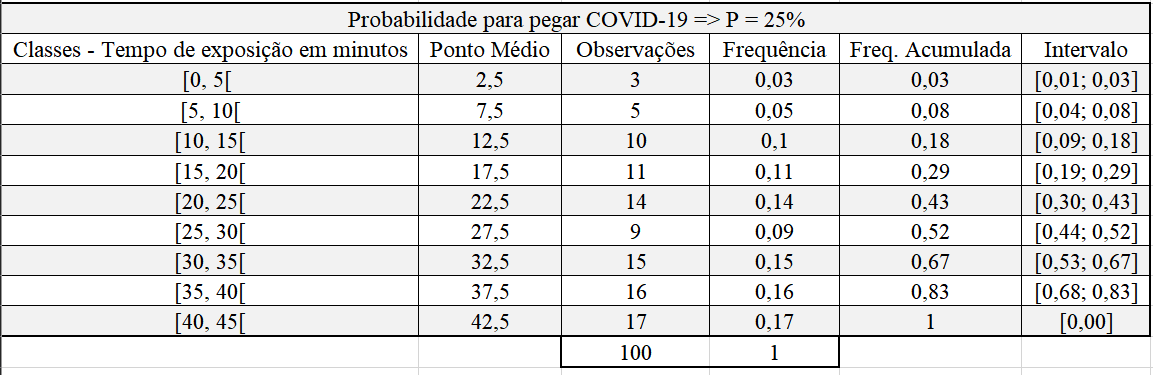
\includegraphics[width=15cm]{MonteCarloPics/montecarlo_fatores_pic1_1.PNG}
    \caption{Fatores: Probabilidade de pegar COVID-19.}
    \label{fig:fat11}
\end{figure}
\FloatBarrier
\FloatBarrier
\begin{figure}[h]
    \centering
    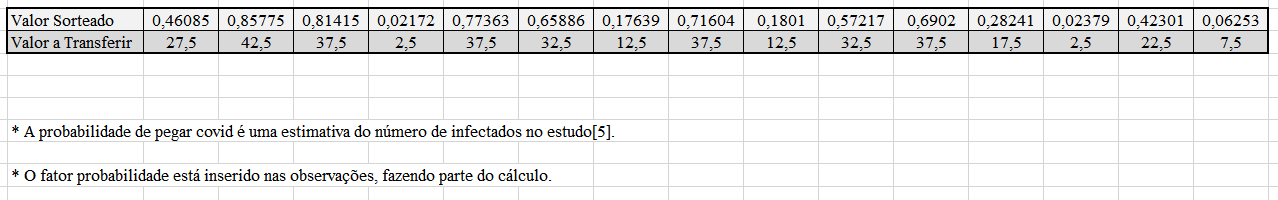
\includegraphics[width=15cm]{MonteCarloPics/remerge/fig2.PNG}
    \caption{Fatores: Classes geradas aleatoriamente para a probabilidade acima.}
    \label{fig:fat12}
\end{figure}
\FloatBarrier
{\it Probabilidade de ter COVID-19 (Figuras 3 e 4):}
\FloatBarrier
\begin{figure}[h]
    \centering
    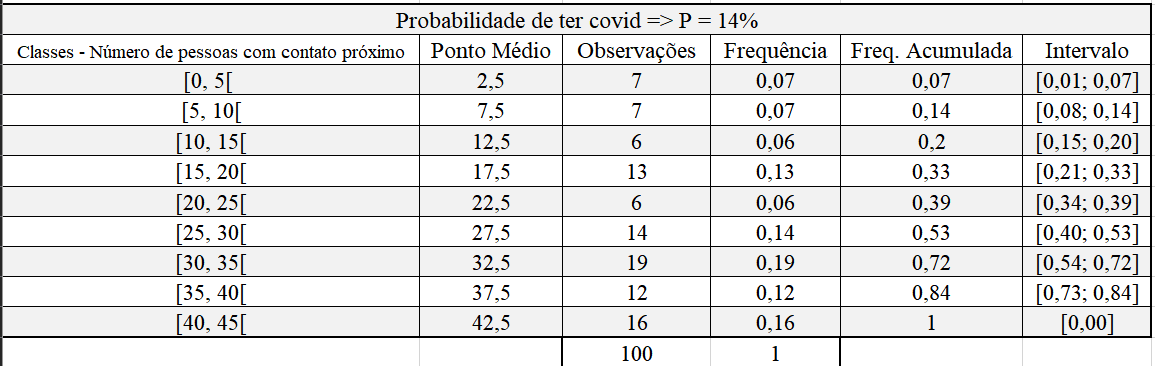
\includegraphics[width=15cm]{MonteCarloPics/montecarlo_fatores_pic2_1.PNG}
    \caption{Fatores: Probabilidade de ter COVID-19.}
    \label{fig:fat21}
\end{figure}
\FloatBarrier
\FloatBarrier
\begin{figure}[h]
    \centering
    
\includegraphics[width=15cm]{MonteCarloPics/remerge/fig4.PNG}
    \caption{Fatores: Classes geradas aleatoriamente para a probabilidade acima.}
    \label{fig:fat22}
\end{figure}
\FloatBarrier
{\it Probabilidade de pegar COVID-19 por proximidade (Figuras 5 e 6):}
\FloatBarrier
\begin{figure}[h]
    \centering
    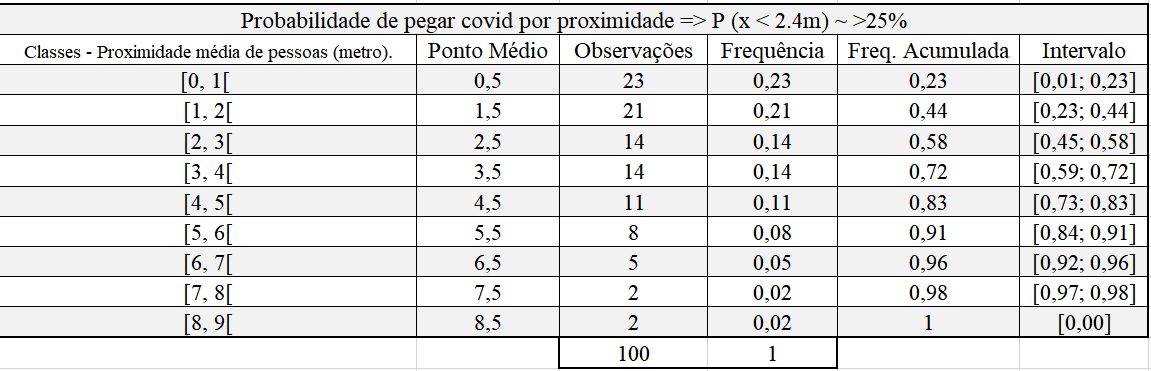
\includegraphics[width=15cm]{MonteCarloPics/montecarlo_fatores_pic3_1.PNG}
    \caption{Fatores: Probabilidade de pegar COVID-19 por proximidade.}
    \label{fig:fat31}
\end{figure}
\FloatBarrier
\FloatBarrier
\begin{figure}[h]
    \centering
    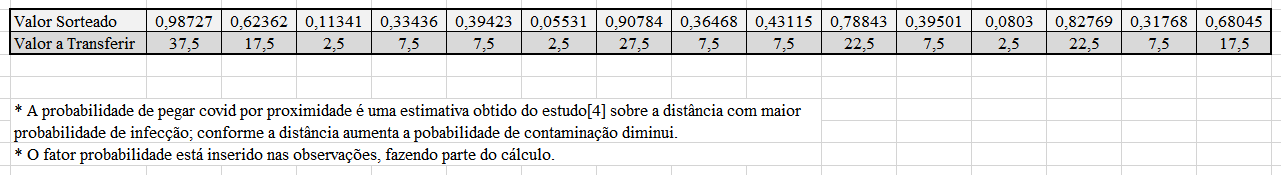
\includegraphics[width=15cm]{MonteCarloPics/remerge/fig6.PNG}
    \caption{Fatores: Classes geradas aleatoriamente para a probabilidade acima.}
    \label{fig:fat32}
\end{figure}
\FloatBarrier

Após a obtenção dos valores para cada probabilidade componente, derivamos 4 probabilidades com base nas interseções destas componentes. Na figura 7, tem-se os valores obtidos para cada uma das 4 novas probabilidades, seguidas de sua descrição e processo de obtenção na figura 8.

\FloatBarrier
\begin{figure}[h]
    \centering
    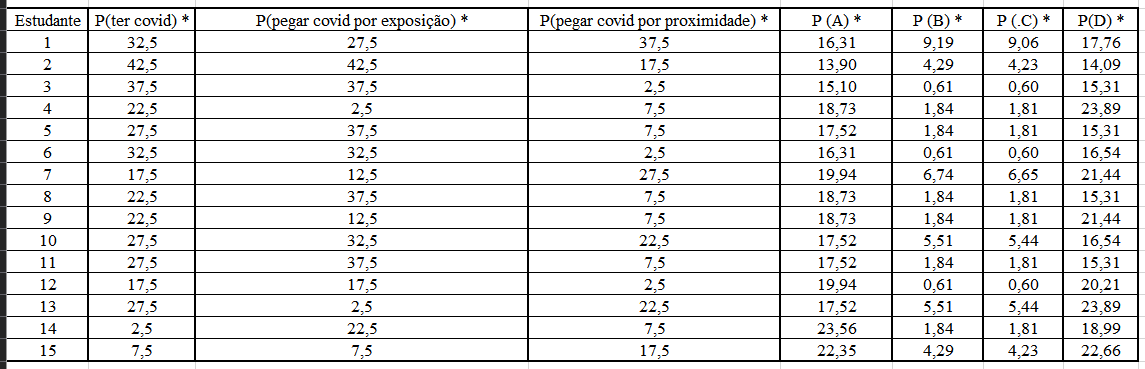
\includegraphics[width=15cm]{MonteCarloPics/remerge/fig7.PNG}
    \caption{Método: Tabela com as probabilidades.}
    \label{fig:met1}
\end{figure}
\FloatBarrier
\FloatBarrier
\begin{figure}[h]
    \centering
    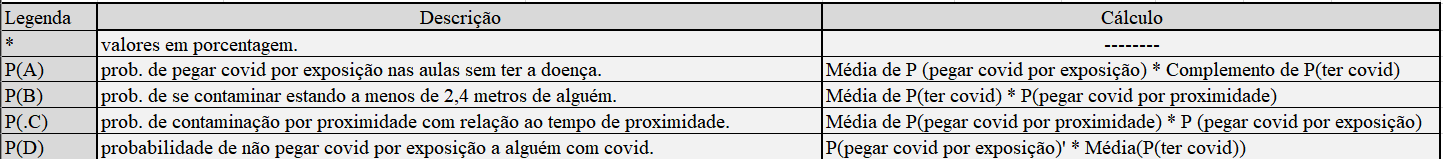
\includegraphics[width=15cm]{MonteCarloPics/montecarlo_pic2.PNG}
    \caption{Método: Legenda.}
    \label{fig:met2}
\end{figure}
\FloatBarrier

Na figura 9, a equipe fez a leitura dos resultados obtidos conforme tinha projetado, bem como a análise entre os resultados e o resultado final.

\FloatBarrier
\begin{figure}[h]
    \centering
    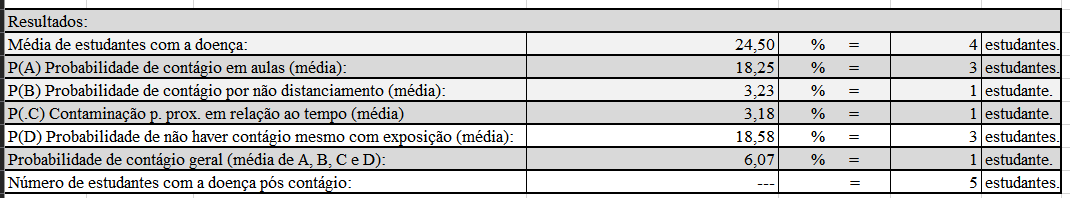
\includegraphics[width=15cm]{MonteCarloPics/remerge/fig9.PNG}
    \caption{Método: Resultados.}
    \label{fig:met3}
\end{figure}
\FloatBarrier

\section{Resultados}

Os resultados obtidos estão apresentados na seção três do artigo (Figura 9), neles estão contidos probabilidades dos estudantes serem contagiados em três cenários diferentes. O número de estudantes expostos a este contexto é 15, sendo que quatro estudantes já estavam contaminados e ocorreu um novo contágio entre os estudantes, resultado no total de cinco estudantes contaminados após o contágio. 

Percebe-se que as probabilidades A e D, contágio durante as aulas e não contrair a doença mesmo exposto respectivamente, mantiveram-se próximas a um quinto da amostra. A análise também indicou que a suscetibilidade à doença (P(B)), mesmo não respeitando o distanciamento, é baixa, mantendo-se inferior a 5\% da amostra; da mesma forma, a probabilidade C, a exposição de um estudante em relação ao tempo em que esteve próxima de um estudante contaminado, manteve-se inferior a 5\% da amostra.

Na obtenção da probabilidade geral, foram levadas conta as probabilidades derivadas. O cálculo desta probabilidade consiste na soma das probabilidades A, B e C menos a probabilidade D, indicando o número de infectados novos no teste. 

\section{Considerações Finais}

A equipe observou que as probabilidades obtidas para a premissa do projeto foram satisfatórias pois o intuito da pesquisa era determinar qual o grau de contágio a retomada as aulas presenciais traria. Portanto, dados os resultados, concluímos que, dado o fato de que 14\% da amostra possui COVID-19 -- isso contabiliza 4 estudantes no teste, a diferença de mais um novo caso (5 estudantes no fim do estudo) foi de impacto inexpressivo, considerando que não houve um cuidado dos alunos com relação a manter o distanciamento (probabilidade b) e ao uso de equipamentos de proteção (que não fizeram parte deste estudo, mas podem ajudar na proteção individual no dia a dia). 
A equipe conclui então que, mesmo observando o evento no seu pior caso e estimando as probabilidades não cumprimento das boas normas de autoproteção, há uma baixa probabilidade de novos contágios (6\% como apontado no estudo).
Deve-se levar em conta que o tamanho da amostra e que outras probabilidades de contaminação mais complexas impactam nos resultados do teste.



\printbibliography  \iffalse Mostra as referências em mybib.bib. \fi

\end{document}

